\documentclass[twoside]{article}

% Fonts + Colors ~~~~

\usepackage{lipsum}
\usepackage{fontspec}
\usepackage{dashrule}
\usepackage[export]{adjustbox}
\usepackage[usenames, dvipsnames]{color}
\usepackage{comment}

\definecolor{Gray}{RGB}{120, 120, 120}
\definecolor{LogoRed}{RGB}{153, 0, 0}
\definecolor{LogoTurquoise1}{RGB}{1, 123, 147}
\definecolor{LogoTurquoise2}{RGB}{0, 158, 171}
\definecolor{LogoTurquoise3}{RGB}{0, 186, 187}
\definecolor{BackgroundBlue}{RGB}{247, 254, 255}
\definecolor{LightBlue}{RGB}{230, 247, 255}
\definecolor{LightRed}{RGB}{231, 103, 97}
\definecolor{DarkGray}{RGB}{71, 71, 71}

\begin{comment}
\newfontfamily\Avenir[
    Path= fonts/,
    Extension= .otf,
    UprightFont = *-45Book,
    ItalicFont = *-45BookOblique,
    BoldFont = *-95Black,
]{AvenirLTStd}

\newfontfamily\TradeGothic[
    Path = fonts/,
    Extension = .otf,
    UprightFont = *-No18,
    BoldFont = *-No20Bold,
]{TradeGothicCondensed}

\setmainfont[Ligatures=TeX]{Avenir}
\Avenir\fontsize{9pt}{12pt}\selectfont

\end{comment}

\usepackage[condensed]{roboto}
\usepackage[default,osfigures,scale=0.95]{opensans}
\usepackage[T1]{fontenc}

\fontsize{9pt}{12pt}\selectfont

% Formatting ~~~~

\usepackage{geometry}

\geometry{
    letterpaper,
    top=1.75in,
    bottom=1.75in,
    inner=0.75in,
    outer=0.75in,
    headsep=1in,
    headheight=0.5in,
    footskip=1in,
    % showframe
}

\usepackage[document]{ragged2e}
\parskip=8pt
\parindent=0pt
\linespread{1.2}
\setlength{\columnsep}{0.75cm}

% \usepackage{sectsty}
% \sectionfont{\fontfamily{pag}\selectfont\color{LogoTurquoise1}\vspace{-\parskip}\Large\uppercase}
% \subsectionfont{\color{LogoTurquoise1}\vspace{-\parskip}\mdseries\Large}

\usepackage{titlesec}
\titleformat*{\section}{\fontfamily{pag}\selectfont\color{LogoTurquoise1}\vspace{-\parskip}\bfseries\Large\uppercase}
\titleformat*{\subsection}{\color{LogoTurquoise1}\vspace{-\parskip}\Large}


% Headers + Footers ~~~~

\usepackage{fancyhdr}
\pagestyle{fancy}

\renewcommand{\sectionmark}[1]{\markboth{#1}{}}
\usepackage{fourier-orns}

\fancyhead{} % clear all header fields
\fancyfoot{} % clear all footer fields
\fancyfoot[LE]{\thepage \hspace{0.4cm} \roboto\selectfont\textcolor{LightRed}{\uppercase{Recruiting the Out-of-State University}}}
\fancyfoot[RO]{\roboto\selectfont\textcolor{Gray}{\leftmark} \hspace{0.4cm} \thepage}
\renewcommand{\headrulewidth}{0pt}

\fancypagestyle{tablepage}{  % No Header, Regular Footer
    \fancyhead{}
    \fancyfoot{}
    \renewcommand\headrule{\hrulefill
\raisebox{-2.1pt}[10pt][10pt]{\quad\decofourleft\decotwo\decofourright\quad}\hrulefill}
}

\addtolength{\skip\footins}{10pt}


% Links + Lists ~~~~

\PassOptionsToPackage{hyphens}{url}\usepackage[colorlinks=true, linkcolor=cyan, urlcolor=blue, citecolor=blue, breaklinks=true]{hyperref}
\newcommand{\superscript}[1]{$^{#1}$}

%reference list stuff
\usepackage[natbibapa]{apacite}

%\usepackage[super,numbers]{natbib}

\makeatletter
\renewcommand\@biblabel[1]{\superscript{#1}}
\makeatother

\renewcommand{\refname}{\vspace{-0.65cm}}

\usepackage{enumitem}
\setlist{nosep, itemsep=0pt, parsep=0pt}

\renewcommand{\labelitemi}{\color{LightRed}$\triangleright$}
\renewcommand{\labelitemii}{\color{LogoTurquoise2}$\cdot$}
\renewcommand\labelitemiii{$\circ$}


% Block Formats ~~~~

\usepackage{mdframed}

\newenvironment{quote-block}{  % quote block
    \begin{quote}
    \roboto\selectfont
    \color{LogoTurquoise2}
}
{
    \end{quote}
}

\newenvironment{color-block}[1][Key Points]{  % text block
    \vspace{0.5cm}
    \begin{mdframed}[backgroundcolor=LightBlue, linecolor=LightBlue, userdefinedwidth=\textwidth, leftmargin=0cm, innerleftmargin=1cm, innerrightmargin=2cm, innertopmargin=0.5cm, innerbottommargin=1cm]
    \color{DarkGray}
    \subsection*{\color{LogoTurquoise1}{\Large#1}}
    \vspace{-0.2cm}
}
{
    \end{mdframed}
    \vspace{0.2cm}
}


% Figures ~~~~

\usepackage{graphicx}
\usepackage{caption}
\usepackage[labelformat=simple]{subcaption}

\DeclareCaptionSubType*{figure}
\renewcommand\thesubfigure{}

\DeclareCaptionFont{CaptionFont}{\roboto\selectfont}
\DeclareCaptionFont{LightRed}{\color{LightRed}}

\captionsetup{labelfont={CaptionFont, LightRed}, figurename=FIGURE, tablename=TABLE}

\newcommand{\addFigure}[4][0.2] {  % Add single figure
\begin{figure}[!ht]
    \vspace{0.45cm}
    \centering

    \includegraphics[width=0.45\textwidth, trim={0 0 0 #1cm}, clip]{images/#2}
    \caption{\roboto\selectfont\textcolor{Gray}{\uppercase{#3}}}
    \label{fig:#4}

\end{figure}
}

\usepackage{stfloats}
\newcommand{\addFigureSet}[4] {  % Add 2x2 figure set
\begin{figure*}[#4]
    \vspace{0.45cm}
    \centering

    \begin{subfigure}[b]{.45\linewidth}
      \includegraphics[width=\linewidth, cfbox=Gray 0.4pt]{images/maps/#1_1}
      \caption{1}
    \end{subfigure}\hfill
    \begin{subfigure}[b]{.45\linewidth}
      \includegraphics[width=\linewidth, cfbox=Gray 0.4pt]{images/maps/#1_2}
      \caption{2}
    \end{subfigure}

    \smallskip

    \begin{subfigure}[b]{.45\linewidth}
      \includegraphics[width=\linewidth, cfbox=Gray 0.4pt]{images/maps/#1_3}
      \caption{3}
    \end{subfigure}\hfill
    \begin{subfigure}[b]{.45\linewidth}
      \includegraphics[width=\linewidth, cfbox=Gray 0.4pt]{images/maps/#1_4}
      \caption{4}
    \end{subfigure}

    \caption{\roboto\selectfont\textcolor{Gray}{\uppercase{#2}}}
    \label{fig:#3}

    \ifnum\pdfstrcmp{#4}{b}=0
      \vspace{-1cm}
    \else
      \vspace{0.45cm}
    \fi

\end{figure*}
}

\newcommand{\addSmallMultiples}[3] {  % Add 3x5 figure set
\begin{figure*}[t]
    \vspace{0.45cm}
    \centering

    \includegraphics[width=0.3\textwidth, cfbox=Gray 0.4pt, trim={0 1cm 0 0}, clip]{graphs/199193/#1}\hfill
    \includegraphics[width=0.3\textwidth, cfbox=Gray 0.4pt, trim={0 1cm 0 0}, clip]{graphs/186380/#1}\hfill
    \includegraphics[width=0.3\textwidth, cfbox=Gray 0.4pt, trim={0 1cm 0 0}, clip]{graphs/196097/#1}

    \smallskip

    \includegraphics[width=0.3\textwidth, cfbox=Gray 0.4pt, trim={0 1cm 0 0}, clip]{graphs/100751/#1}\hfill
    \includegraphics[width=0.3\textwidth, cfbox=Gray 0.4pt, trim={0 1cm 0 0}, clip]{graphs/106397/#1}\hfill
    \includegraphics[width=0.3\textwidth, cfbox=Gray 0.4pt, trim={0 1cm 0 0}, clip]{graphs/110635/#1}

    \smallskip

    \includegraphics[width=0.3\textwidth, cfbox=Gray 0.4pt, trim={0 1cm 0 0}, clip]{graphs/110653/#1}\hfill
    \includegraphics[width=0.3\textwidth, cfbox=Gray 0.4pt, trim={0 1cm 0 0}, clip]{graphs/201885/#1}\hfill
    \includegraphics[width=0.3\textwidth, cfbox=Gray 0.4pt, trim={0 1cm 0 0}, clip]{graphs/126614/#1}

    \smallskip

    \includegraphics[width=0.3\textwidth, cfbox=Gray 0.4pt, trim={0 1cm 0 0}, clip]{graphs/139959/#1}\hfill
    \includegraphics[width=0.3\textwidth, cfbox=Gray 0.4pt, trim={0 1cm 0 0}, clip]{graphs/155317/#1}\hfill
    \includegraphics[width=0.3\textwidth, cfbox=Gray 0.4pt, trim={0 1cm 0 0}, clip]{graphs/166629/#1}

    \smallskip

    \includegraphics[width=0.3\textwidth, cfbox=Gray 0.4pt, trim={0 1cm 0 0}, clip]{graphs/181464/#1}\hfill
    \includegraphics[width=0.3\textwidth, cfbox=Gray 0.4pt, trim={0 1cm 0 0}, clip]{graphs/215293/#1}\hfill
    \includegraphics[width=0.3\textwidth, cfbox=Gray 0.4pt, trim={0 1cm 0 0}, clip]{graphs/218663/#1}

    \caption{\roboto\selectfont\textcolor{Gray}{\uppercase{#2}}}
    \label{fig:#3}
\end{figure*}
}


% Tables ~~~~

\usepackage[figuresright]{rotating}
\usepackage{multirow}
\usepackage[table]{xcolor}

\usepackage{etoolbox}
\AfterEndEnvironment{table-env}{\restoregeometry\twocolumn}

\newenvironment{table-env}[3][10]{
  \clearpage
  \newgeometry{top=0.5in, bottom=1in, inner=0.75in, outer=0.75in, footskip=0.25in}
  \begin{sidewaystable}
  \fontsize{8pt}{#1pt}\selectfont
  \ifnum\pdfstrcmp{#2}{x}=-1
    \rotatebox[origin=c]{270}{\begin{minipage}{\textwidth}\caption{\roboto\selectfont\textcolor{Gray}{\uppercase{#2}}}\label{tbl:#3}\end{minipage}}
  \fi
}
{
  \end{sidewaystable}
  \clearpage
}

\newcommand{\addTable}[4][p] {  % Add Table

\begin{table*}[!hb]

    \ifnum\pdfstrcmp{#1}{l}=0
      \begin{sideways}
    \fi

    \centering

    \begingroup
      \fontsize{8pt}{10pt}\selectfont
      \input{tables/#2.tex}
    \endgroup

    \ifnum\pdfstrcmp{#1}{l}=0
      \end{sideways}
    \fi

    \vspace{0.2cm}
    \caption{\roboto\selectfont\textcolor{Gray}{\uppercase{#3}}}
    \label{tbl:#4}

    \vspace{-1cm}

\end{table*}

}


\usepackage{Sweave}
\begin{document}
\sloppy

\Sconcordance{concordance:joyce_report_discussion_oj.tex:joyce_report_discussion_oj.Rnw:%
1 4 1 1 0 4 1 1 18 189 1}



% Title Page ~~~~

\pagecolor{BackgroundBlue}
\newgeometry{top=0cm, bottom=0cm, left=0cm, right=0cm}
\begin{titlepage}

        \makebox[0pt][l]{%
          \raisebox{-0.49\totalheight}[0pt][0pt]{%
          \scalebox{-1}[1]{
            
\includegraphics[width=9in]{./images/layer.png}}}}%

        \hspace{-0.7cm}
        \makebox[0pt][l]{%
          \raisebox{-1.43\totalheight}[0pt][0pt]{%
            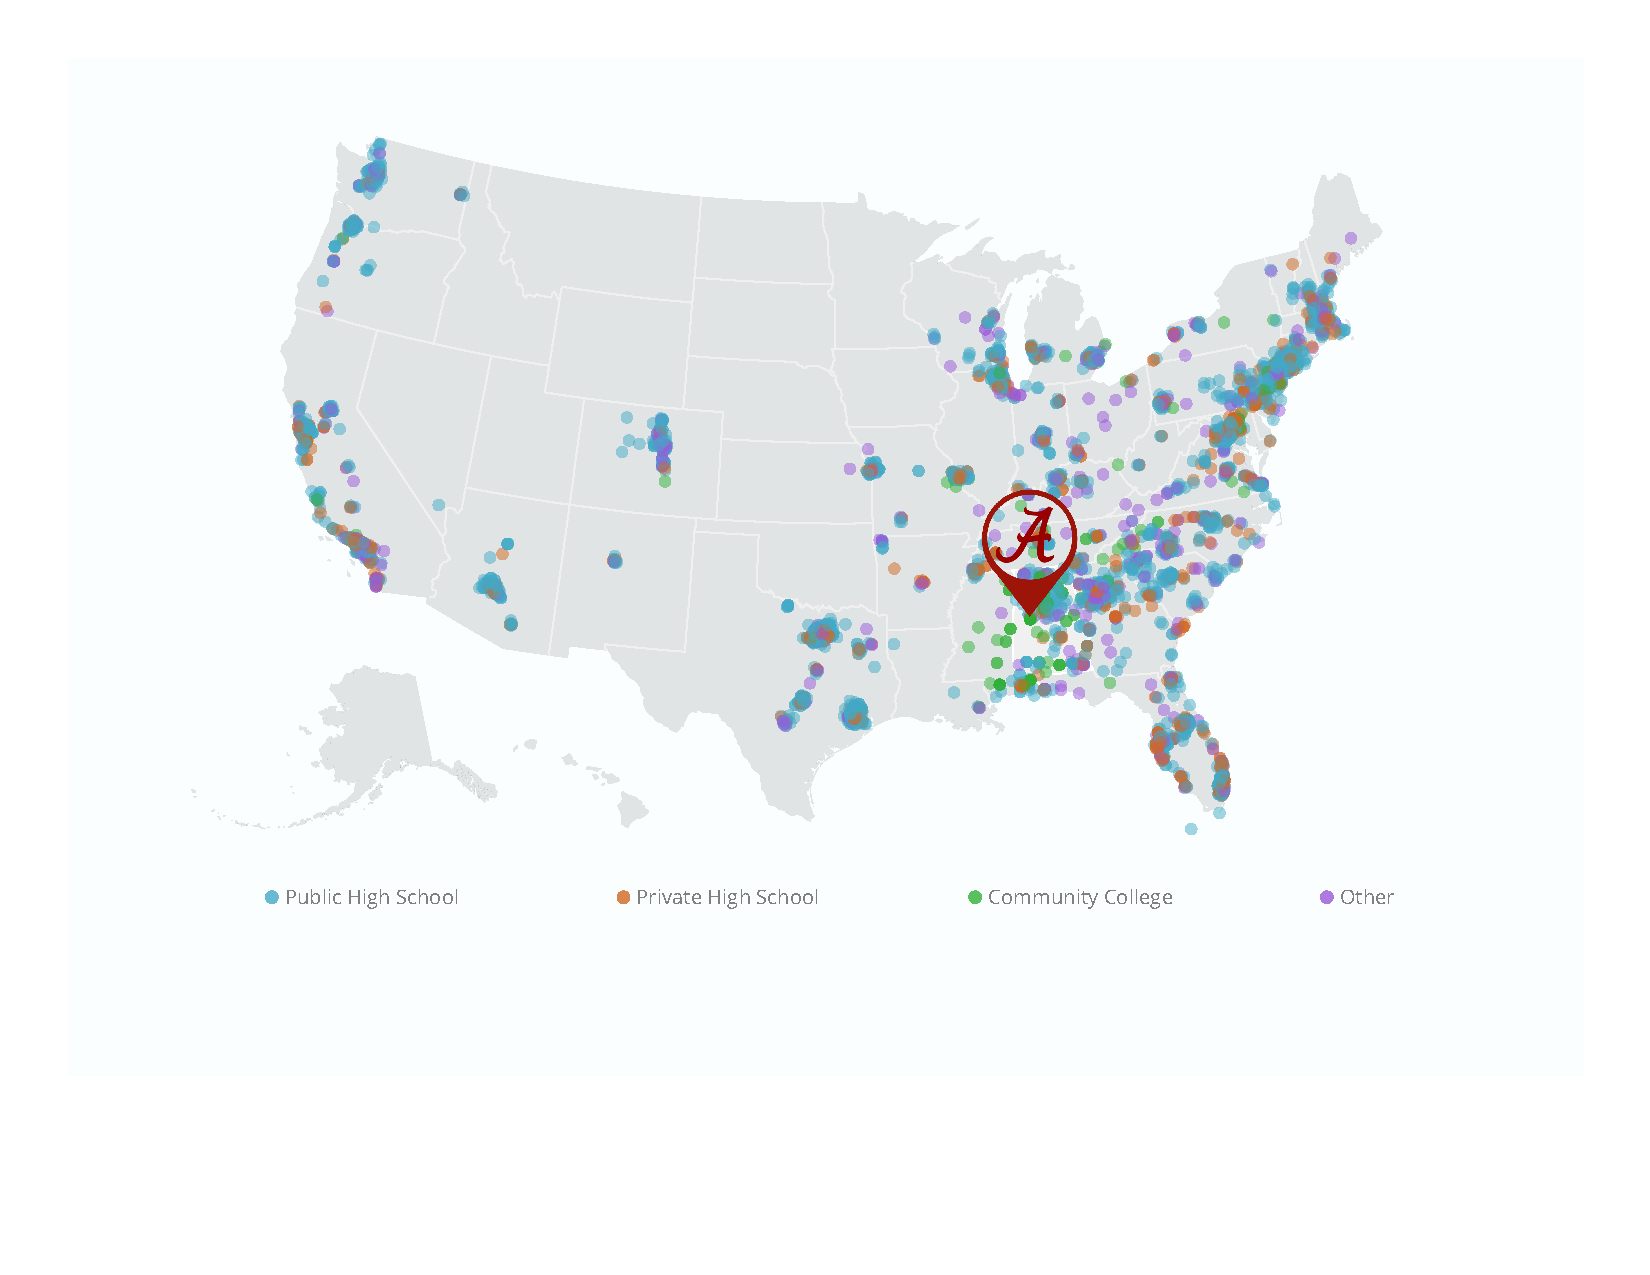
\includegraphics[width=9in, trim={2cm 0 2cm 2cm}, clip]{./images/map_ua.pdf}}}%

        \makebox[0pt][l]{%
          \raisebox{-1.44\totalheight}[0pt][0pt]{%
            
\includegraphics[width=9in]{./images/layer.png}}}%

        \centering\color{DarkGray}\fontsize{30}{60}

        \vspace{0.3cm}
        \hdashrule{0.8\textwidth}{1pt}{1pt} \\

        \vspace{0.8cm}
        \textbf{\color{LogoRed}{RECRUITING}} \\
        \vspace{0.2cm}
        \textbf{\color{LogoRed}{THE OUT-OF-STATE UNIVERSITY}}

        \vspace{0.2cm}
        \Large\textit{\fontfamily{pag}\selectfont Off-campus recruiting by public research universities} \\

        \vspace{0.3cm}
        \hdashrule{0.8\textwidth}{1pt}{1pt} \\

	\vspace{17.1cm}
        \large Crystal Han \\
        Ozan Jaquette \\
        Karina Salazar \\~\\
        %\textit{\color{Gray}{March 2019}}

\end{titlepage}

% Blank Page ~~~~
 
\pagecolor{LightBlue}
\begin{titlepage}
    \color{LightBlue}{x}
\end{titlepage}

% Begin Template ~~~~

\pagecolor{white}
\restoregeometry
\setcounter{page}{1}
\twocolumn

\parskip=14pt
\linespread{1.3}


\section*{Discussion and Implications for Policy and Practice\markboth{Discussion}{}}

\subsection*{Summary}

This study investigated off-campus recruiting visits by public research universities, which we argue are indicators of university enrollment priorities.  The majority of universities in our sample made more than twice as many out-of-state recruiting visits than in-state recruiting visits.  These out-of-state visits focused primarily on public schools in affluent, predominantly White communities and with a disproportionate focus on predominantly White private schools.  

%University recruiting behavior is an indicator of enrollment priorities [CUT THIS SENTENCE AND MOVE BELOW?].  This study suggests that the recruiting behavior and enrollment priorities of many public research universities biased against state residents, low-income communities, and [TO A LESSER EXTENT?] communities of color.  
Our data indicate that most universities did not visit the majority of public high schools in their home state. This finding is not an indictment; universities in large, populous states with formalized statewide higher education systems (e.g., the State University of New York) cannot be expected to visit every high school. Nevertheless, some universities  -- notably those that receive stronger state funding -- covered their home state more thoroughly and more equitably than others.  For example, The University of Nebraska-Lincoln visited most public high schools in Nebraska. SUNY-Stony Brook visited most public high schools in its ``home'' jurisdiction of Long Island. Both NC State and UC-Irvine made more in-state recruiting visits than out-of-state visits and these in-state visits did not exhibit socioeconomic or racial bias.  

By contrast, many universities that focused recruiting efforts on out-of-state schools did a poor job of covering their home state. Some state flagships visited a small proportion of public high schools despite being in less populous states with relatively few public high schools (e.g., University of Alabama, University of Kansas, University of Georgia).  Other state flagships showed pronounced socioeconomic and racial bias in in-state recruiting visits (e.g., UC-Berkeley, OTHER).

\subsection*{Rethinking Policy Discourse on Access}

Mainstream policy discourse about access inequality draws heavily from scholarship by economists and places responsibility on students and K-12 schools rather than universities. For example, the 2014 White House ``Access Summitt'' comissioned a literature review of the causes of access inequality \citep{RN4016}.  This review highlighted the ``achievement gap'' and ``under-matching'' -- the idea that high-achieving, low-income students do not apply to selective colleges because they do not obtain information and guidance about college choices at home or at school \citep{RN3699,RN3700}.  Economic theory rationalizes access inequality due to the achievement gap based on the idea that the most talented students make the most of learning opportunities afforded by universities with superior resources \citep{RN1549,RN2247,RN2402,RN1545}. By contrast, under-matching is antithetical to economic theory because the best "inputs" are not going to the best college. In turn, the under-matching literature has motivated dozens of interventions designed to change student behavior by providing information and guidance \citep[e.g., ][]{RN4352,RN4345,RN4351}.  
%Economic theory rationalizes access inequality due to the achievement gap based on the idea that the most talented students should be matched to institutions that spend the most per student because these students make the most of learning opportunities afforded by superior resources \citep{RN1549,RN2247,RN2402,RN1545}.

Our findings about off-campus recruiting suggest an alternative explanation for under-matching. \cite{RN4324} shows that under-represented student populations are particularly sensitive to which universities take time to visit their high school.  For many states, our findings paint a picture of poor or majority-minority high schools being unlikely to receive a recruiting visit from the state flagship university. Similarly, Means \cite{RN4420} analysis of rural students at a predominantly African American high school in Georgia found that the milistary and local technical college were the only institutions that visited their high school. By contrast, affluent high schools are more likely to receive visits from their state flagship university and from selective public and private universities from across the country.  When students attend a high school that does not receive a visit from a university, they are less likely to know the university is an option.  Therefore, the recruiting patterns we observed create information asymmetries that are strongly related to race and class.  These recruiting patterns also create differences in the extent to which students ``feel wanted'' -- by specific universities and by higher education in gneral -- that are correlated with race and class \citep{RN4324}.  Given these findings, we suggest that ``under-matching'' may often be caused by ``under-recruiting'' rather than lack of guidance.
%an analysis of access to higher education for African American students in rural Georgia by Means [CITE] found that many students with baccalaureate aspirations eventually chose the military or community colleges in part because these were the institutions that visited their high school.
%Similarly, the publication of our New York Times op-ed on off-campus recruiting [LINK] evoked Tweets like ``I didn't learn until recently that colleges visit high schools, because we only ever saw the army'' and ``We occasionally had local college recruiters drop by occasionally, but mostly military or votech.''  Our research finds that many public research universities fail to visit poor, minority, and rural schools because they focus recruiting efforts on affluent communities.  
%tweet 1 https://twitter.com/iff_or/status/985946720935731200
%tweet 2 https://twitter.com/gizm0_0/status/985948440071847936
%If talented students attending schools in poor, minority communities primarily see recruiters from for-profit colleges and the military while students at affluent schools receive visits from flagship universities across the country, then should re-frame the problem of high-achieving low-income students not being aware of their options or not feeling like they belong at a public flagship university as an ``under-recruiting'' problem rather than a problem caused by lack of guidance.


While recruiting behavior affects student opportunities, our research analyzes recruiting behavior as a means of gaining insight about university enrollment priorities.  Mainstream policy discourse assumes that universities are passive recipients of applications or are progressive actors doing their best to increase access in spite of the deficiencies of students and K-12 schools \cite{RN4016, RN4017}.  The implicit assumption here is that doubling the number of applications from high-achieving low-income students will double their enrollment. By contrast, our analyses suggests that the majority of public research universities prefer a mostly-affluent student body. 

In particular, our findings coalesce with a growing enrollment management literature \citep[e.g., ][]{RN3685,RN3528,RN4409,RN4032} to suggest that many public research universities prioritize affluent, non-meritorious, out-of-state students. Aside from a handful of prestigious universities (e.g., University of Michigan), most public research universities universities (e.g., University of South Carolina, University of Alabama) compete for out-of-state prospects who could not gain admission to flagship public universities in their home state.  Indeed, many public research universities have adopted institutional ``merit'' aid programs that target out-of-state prospects with moderate academic achievement \citep{RN1469,RN3762,RN4032,RN4409}. These students do not take advantage of the unique opportunities public research universities offer.  Meanwhile, high-achieving, low-income students are often diverted to regional state colleges and community colleges, which have lower resources and offer fewer learning opportunities than public research universities.  This is not a meritocracy.  As a consequence of the shift in enrollment priorities from merit to revenue, public research universities make diminished contributions to economic and civic development because they do not prioritize enrolling students with the most talent.
%Meanwhile, high-achieving, poor state residents are increasingly diverted to institutions that do not maximize their potential [CITE]. 

Policy efforts that focus solely on changing student behavior (the ``demand side'') will fail to yield substantial increases in enrollment from under-represented student populations if they are not accompanied by policies that create incentives for universities to enroll these students (the ``supply side'').  For example, the under-matching literature has spawned a new population of ``matching'' organizations (e.g., QuestBridge, CollegePoint), which identify high-achieving, low-income students, reach out to these students and match them to selective colleges and universities which promise to provide four-year full scholarships.  These organizations increase the ``quality'' of match between students and colleges but there is no reason to believe that these organizations increase the total number of low-income students that selective institutions are willing to enroll.
%Therefore, policy efforts that focus solely on changing student behavior (the ``demand side'') will fail to yield substantial increases in enrollment from under-represented student populations because many universities value consumer purchasing power over merit.  

\subsection*{State Policy Implications}

\textbf{\textit{State funding and university enrollment priorities}}. The transformation of enrollment priorities at public research universities is a response to a broken system of postsecondary education finance, led by state disinvestment in public universities.  While state cuts to public research universities are often rationalized on the grounds that these organizations can generate alternative revenue sources [CITE], the unintended consequence is that universities respond by prioritizing students that generate the most net tuition revenue.  \cite{RN3753} found that public research universities responded to state funding cuts by growing nonresident enrollment. Nonresident enrollment growth is not simply a function of enjoying excess demand and letting in more applicants; rather, our research shows that many universities aggresively incite nonresident enrollment demand by focusing recruiting efforts on out-of-state students.
%\cite{RN2535} suggests that public research universities can grow nonresident enrollment simply by admitting more applicants because these institutions enjoy excess demand from nonresident students. 

Our results suggest a strong relationship between state support and university recruiting behaviors.  Broadly speaking, universities with the least state funding tended (e.g., University of Alabama, Rutgers, University of South Carolina) focused recruiting efforts on out-of-state communities, visited relatively few in-state high schools, and exhibited socioeconomic and/or racial bias in in-state recruiting visits.  By contrast, universities with relatively generous state funding (e.g., NC State, OTHERS?) tended to have best records of in-state coverage and smaller focus on out-of-state students. [KARINA MODIFY PARAGRAPH TO REFLECT MOST UP TO DATE RESULTS]

These findings raise important normative policy questions about public research universities and the public good. Should public research universities conceive of the public good in terms of serving the state -- including the historic mission of social mobility for state residents -- the nation, or the world? Or should public research universities focus on pursuing their self-interest (e.g., prestige, revenue generation) rather than providing value to society? However, statements about what the mission of public universities \textit{should} be have little effect on organizational behavior. Rather, borrowing the old adage,
``he who pays the piper calls the tune.'' Our results suggest that if state policymakers want public research universities to prioritize access for meritorious state residents -- particularly students from poor communities and communities of color -- they must increase state funding.

%Therefore, if state policymakers want public research universities to prioritize access for meritorious state residents, the state must invest in public research universities.

%Public research universities were founded with two broad goals \citep{RN2269,RN1149}: first, to provide opportunity to meritorious state residents who cannot afford tuition at private institutions; and, second, to contribute to the economic and civic development of the state, with public research universities designated the special role of training future business, professional, and political leaders of the state.  In comparison to regional state colleges and community colleges, public research universities spend more resources per student and, in turn, confer greater learning and career opportunities \citep{RN1545}. 

Increased state support could come in the form of more generous state appropriations.  Prior research finds that growth in state appropriations increases access by placing downward pressure on resident tuition price \citep{RN2609} which, in turn, positively affects student demand \citep{RN3068}.  On the supply side, more generous state appropriations enables universities to be less reliant on tuition revenue from affluent students, thus incentivizing universities to enroll more low-income students.

Increased financial support could also come in the form of more generous federal or state need-based grant aid programs, which also affects both student demand and university supply. Grant aid increases student demand by reducing net price paid.  On the supply side, more generous need-based grant aid increases the purchasing power of low-income students, incentivizing universities to enroll more low-income students because these students now generate more net tuition revenue and require less need-based institutional aid. If federal and state policymakers are unwilling to increase need-based grant aid, income-share agreements (ISAs) are a non-governmental approach to increasing the purchasing power of poor students. 
%[SAY SOMETHING ABOUT ISAs?] https://www.economist.com/finance-and-economics/2018/07/19/income-share-agreements-are-a-novel-way-to-pay-tuition-fees
%Do you know of a published paper that examined the effect of increased pell grant funding by Obama administration on college enrollment? And ideally decomposing the extent to which effect was driven by increase in student demand or change in supply-side behavior [universities more willing to enroll low-income students because they now have greater purchasing power].

Substantially increasing state spending on higher education is a tough ``ask'' because state budgets face demands from many worth causes \citep{RN1652} and because many states have enacted policies that make it difficult to raise taxes \citep{RN1646}.  However, recent midterm elections changed state legislatures and governors across the country.  Perhaps these changes in state political environment -- coupled with mounting evidence about the consequences of forcing public universities to rely on paying customers -- will compel states to re-invest in public higher education.

Non-resident enrollment caps are another tool state policymakers can use to ensure that public research universities serve state residents.  For example, North Carolina caps nonresident enrollment at X\% [CITE].  Responding to pressure from state legislators, the  University of California (UC) System proposed to cap out-of-state enrollment at 20\% system-wide \citep{RN4247}.  Compared to other universities in our sample, NC-State, UC-Irvine, and UC-Berkeley focused recruiting visits on their home state, suggesting that non-resident enrollment caps affect university enrollment behaviors. However, we argue that nonresident enrollment caps should be contractually tied to an agreement that the state provides sufficient funding. This way, the responsibility of public universities to serve state residents depends on state responsibility to provide adequate funding to pay for the costs of educating state residents.  Without such an agreement, states may simultaneously defund public research universities and forbid them from replacing state funds with nonresident tuition revenue, thereby resulting in fewer resources per student and a lower quality of education \citep{RN532}.

\textbf{\textit{Funneling students to community colleges}}. Many states (e.g., X, X) have sought to increase baccalaureate attainment by growing community college enrollment and strengthening the transfer function. In California, for example, legislators have pressured the UC system to enroll more community colege transfer students [CITE]. Additionally, several states (e.g., X ) and large metropolitan (e.g., X ) areas have sought to increase college access by adopting free tuition programs for community college students [CITE NCSL].  
%California provides one example of recent policy trends. Here, state legislators have have pressured the University of California (UC) system to enroll more transfer students and UC campuses have complied with this demand [CITE].  
%National Conference of State Legislatures (2016): "Free Community College," Tech. rep.
%This policy trend serves the interests of state policymakers, who can claim that they are giving students an opportunity to obtain a BA from a prestigious UC campus.  This policy trend also serves the interests of UC campuses, who point to the growth of community college transfers as evidence of their commitment to access [CITE]. 

%But empirical evidence unequivocally asserts that attempting to increase BA attainment through community college transfer is bad policy.  

Although community colleges positively affect credential attainment and earnings of students who would otherwise not have attended postsecondary education \citep[e.g., ][]{RN4404}, empirical research unequivocally finds that they are a uniquely bad instrument for increasing BA attainment. 81\% of first-time community college students aspire to obtain a BA \citep{RN4406}. However, only 33\% of degree-seeking students transfer to a 4-year university within six years \citep{RN4406} andonly 14\% of these students earn a BA within six years, compared to 60\% of degree-seeking students who start at a 4-year university \citep{RN4406}.  This negative relationship is causal; econometric analyses consistently find that starting at a community college as opposed to a 4-year institution dramatically lowers the probability of obtaining a BA. \citep[e.g., ][]{RN4284,RN2261,RN4292,RN4405}. The most recent, cutting-edge research by \cite{RN4404} finds starting at a community college rather than a 4-year university reduces probability of getting a BA by 18 percentage points (e.g., from a 50\% probability to 32\% probability).  No other policy intervention to affect BA attainment approaches this level of magnitude.

Further, there are great socioeconomic and racial inequities in which students transfer to state flagship universities \citep{RN1492,RN4406}. In California, a disproportionate number of transfers to the UC system were enrolled in community college honors programs [CITE]. These honors programs guarantee admission to a UC campus if students meet academic achievement requirements [CITE], but access to honors programs is racially and socioeconomically stratified [CITE].  Therefore, this policy trend of funneling BA aspirants to community colleges and pressuring public universities to enroll more transfer students begins to feel like a shell game designed to benefit all the players except low-income students and communities of color. Policymakers can claim they are giving stduents an opportunity to obtain a BA, UC campuses can point to growth in community college transfers as evidence of their commitment to access, and community colleges enjoy enrollment growth. However, starting at a community college dramatically lowers the probability of obtaining a BA and the socioeconomic and racial inequities in access to community college honors programs which guarantee admission to the UC system suggest that UC campuses are skimming the cream rather than providing opportunity to students who have faced the greatest obstacles to college access.  Furthermore, our results suggest that for some universities (e.g., UC-Berkeley), trumpeting the growth in community college transfers provides political cover for concentrating high school visits in affluent communities.  

Therefore, if state policymakers are serious about increasing BA attainmnent for under-represented students, they can no longer feign ignorance of the empirical fact that community colleges are terrible vehicles for BA attainment. Rather, state policies should systematically funnel college-ready high school graduates with BA aspirations into 4-year institutions, a shift that would require investments in the enrollment capacity of public universities.

\subsection*{Implications for university leaders}

Although results indicate a relationship between state funding and university recruiting behavior, several universities facing similar environmental conditions exhibited substantially different recruiting patterns. For example, compared to UC-Berkeley, UC-Irvine did a much better job prioritizing low-income and majority-minority high schools in California despite receiving less state revenue per student than UC-Berkeley. Additionally.  Additionally, UC-Irvine made only 168 out-of-state visits comapred to 421 by UC-Berkeley and out-of-state visits by UC-Berkeley were more focused on affluent, predominantly White high schools.  These findings show that university enrollment priorities and recruiting behaviors are choices made by leadership rather than mere functions of the state external environment. 
%For example, the University of Nebraska and the University of Georgia receive about the same amout of state revenue per FTE student. However, the University of Nebraska visited nearly every public high school in the state, while University of Georgia visited only 35\% of in-state high schools and were more likely to visit affluent high schools than poor ones. 

Recent research by \cite{RN4408} found that aggressive outreach combined with the promise four years of free tuition and fees dramatically increased applications and enrollment at the University of Michigan by high-achieving, low-income state residents.  These findings prove that public research universities can dramatically increase the enrollment of low-income state residents if they direct resources towards this goal. Therefore, the problem is not a lack of qualified low-income students. The problem is a lack of will by universities to enroll these students. While all public research universities espouse a commitment to access and equality of opportunity for state residents, our findings suggest that this commitment is largely a public relations effort for many universities. The time is now for university leaders to put their money where their mouth is rather than putting their money where the money is.  Failure to do so will only strengthen the vicious cycle of state disinvestment, university disinvestment in state residents, followed by further state disinvestment as a response to universities no longer serving the state.
%Alternative: The problem is not lack of qualified low-income students. Rather, the problem is lack of will by universities to put their money where their mouth is.
%The time is now for public research universities to ressurect their historic role as the state's preeminent engine of opportunity and social mobility.  

Additionally, public research universities should prioritize enrolling racially and socioeconomically diverse cohorts of state residents because of the consequences for campus culture. Compared to resident students, nonresident students are more affluent, are less likely to be Black or Latinx, and often have lower levels of academic achievement in high school \citep{RN3685}.  Further, recent growth in nonresident at public research universities students is associated with declines in the share of Pell recipients and under-represented minority students \citep{RN3685}.  An extensive literature shows that low socioeconomic and racial diversity negatively affects that academic and social experiences of poor students and students of color \citep[e.g., ][]{RN3205,RN3193,RN3639,RN3185} and negatively affects learning outcomes for \textit{all} students \citep[e.g., ][]{RN3026,RN2576,RN3153,RN3174}. \cite{RN4231} show that enrolling large cohorts of affluent, predominantly White students with mediocre records of academic achievement create a campus culture where first-generation college students are chastised for trying hard in class and socially ostracized for their lack of financial resources.  Considering the growth in ``merit'' aid for out-of-state students with mediocre academic achievement [CITE] and our finding that most universities concentrate recruiting efforts on affluent, predominantly White, out-of-state communities, we argue that university enrollment management behaviors are explicitly creating a campus culture that is hostile to poor students and students of color.

Finally, university leaders genuinely concerned about access should make this priority clear to enrollment managers and play a role in the implimentation of enrollment management policies.  Several university presidents and trustees who read our New York Times op-ed [LINK] about off-campus recruiting expressed surprise when confronted with the recruiting patterns of their university.  These anecdotes suggests that trustees and presidents set broad enrollment goals and delegate the achievement of these goals to enrollment management offices and the consulting firms they hire. Enrollment managers may conclude, for example, that the most effective means of satisfying orders from above is targeting affluent out-of-state high schools and pursuing racial diversity by visiting magnet schools but ignoring traditional public schools in communities of color.  Therefore, university leaders must consider how broad enrollment goals create behavioral incentives for enrollment management offices.


\subsection*{Implications for access advocates and future research}

Although we initiated research on university recruiting behavior with the goal of shifting national policy debates about access inequality, an unanticipated effect is that a handful of local actors (e.g., at Emory University, University of Colorado-Boulder) began using our data to initiate discussions with university leadership about enrollment priorities and recruiting behaviors.  These unexpected anecdotes helped us envision a new theory of change, one that operates at the local organiation-level rather than the macro policy-level.

All public universities have local constituents -- both internal and external to the organization -- who care about access and demand that university leaders place a higher priority on access.  Consistent with findings from broader literatures on organizational behavior \citep{RN2436}, universities typically respond to stakeholder demands with lofty rhetoric and by adopting new policies or programs (e.g., holistic admissions, ``no loan'' tuition policies, ``outreach'' efforts) \citep[e.g., ][]{RN4017}.  Often, stakeholders cannot determine whether these responses are earnest or ceremonial. Without concrete evidence that an organizational response is symbolic, stakeholders feel compelled to accept the organizational response and demands for change lose energy

Therefore, our theory of local change is to empower access advocates by collecting concrete, quantifiable data about university recruiting behaviors. These data yield insight about whether university commitments to access are earnest or ceremonial.  Since the data we collect are public, we can release these data to the public. In turn, access advocates can present these data to university leadership when demanding stronger action on access.  Armed with systematic data about university recruiting behavior, access advocates will no longer be pacified by lofty rhetoric or opaque programs with unclear resources.  Therefore, these data provide the foundation for debate about what the university actually does rather than a debate about what the university says it does.

While off-campus recruiting encompesses only one facet of university recruiting efforts, presenting concrete data to university leadership raises the bar for what counts as evidence and shifts the burden of proof to the university. If university leaders claim other recruiting efforts (e.g., ``outreach,''  direct mail) target populations ignored by off-campus recruiting, access advocates can demand concrete, data about these efforts. If leadership cannot produce these data, there is no reason to believe that inequities observed in off-campus recruiting visits are unrepresentative of other recruiting efforts. 

We hope that our data on recruiting behavior is utilized by both internal and external stakeholders concerned with access.  Offices of diversity, equity, and inclusion are particularly well positioned; these offices are charged with creating an inclusive campus climate but our data shows that university recruiting behavior is often antithetical to the representational diversity necessary for an inclusive campus climate.  Other potential internal stakeholders include faculty senates, student groups, and board of trustee members.  The power of an external stakeholder to demand change is a function of university dependence on resources controlled by the stakeholder \citep{RN959}. From this perspective, universities are particularly sensitive to demands from donors and from elected officials who control public funding and policies that regulate university behavior.  Alumni are often well-represented on internal and external committees that have authority over university actions.  Additionally, journalists, community organizers, and non-profit organizations have capacity to inform public opinion and influence elected officials.

Finally, researchers create an empirical basis for local and national policy debates by collecting, analyzing, and disseminating data.  Our research on off-campus recruiting stands on the shoulders of giants, particularly groundbreaking scholarship sociologists \citep[e.g., ][]{RN3519,RN4407,RN4324}. These studies tend to broad in scope -- e.g., encompassing the recruiting, admissions, and yield process -- and are based on qualitative, ethnographic, and archival data from one or two organizations. By contrast, our research collects quantitative data on one facet of university recruiting from a larger number of organizations. A limitation of our research is that we ignore many recruiting interventions utilized by universities because collecting systematic data about one recruiting intervention is so time-intensive. However, policy debates tend to be swayed more by quantitative data from many organizations than qualitative data from one organization. Therefore, we see great potential to inform policy debates by developing a set of successive studies, each collecting systematic, quantifiable data about a particular recruiting intervention. Over time, this research agenda will encompass the breadth of university recruiting behavior.  

We have initiated several new data collections to capture the different means universities utilize to identify and target prospects.  For example, we are using public records request to examine which student characteristics universities prioritize when purchasing the contact information of ``prospects'' from College Board and ACT.  Second, following \cite{RN4331} and \cite{RN4360}, we are developing experimental audit studies to examine how universities respond to ``inquiries'' from prospects with different characteristics? Third, to what extent are university ``outreach'' and ``pipeline'' efforts marginal versus substantial in scale? For each of these data collections, we intend to make the results publicly available so that stakeholders can use these results to push for change at their local university. We also plan to publicly release all data we collect so that researchers and non-profit organizations can conduct their own analyses.  Our hope is that a critical mass of scholars and policymakers become interested in university enrollment management behaviors.  Once this happens, policy debates about access will shift from a focus on student ``deficiencies'' towards a focus on university enrollment priorities.  In turn, policy debates will consider solutions to reduce biases in university enrollment priorities.
%THORNHILL \cite{RN4360}

% References ~~~~

\clearpage
\section*{References\markboth{References}{}}
\titleformat*{\section}{\color{white}\vspace{-50pt}\centering}

\bibliographystyle{apacite}
\def\bibfont{\small}
\expandafter\def\expandafter\UrlBreaks\expandafter{\UrlBreaks%
  \do\a\do\b\do\c\do\d\do\e\do\f\do\g\do\h\do\i\do\j%
  \do\k\do\l\do\m\do\n\do\o\do\p\do\q\do\r\do\s\do\t%
  \do\u\do\v\do\w\do\x\do\y\do\z\do\A\do\B\do\C\do\D%
  \do\E\do\F\do\G\do\H\do\I\do\J\do\K\do\L\do\M\do\N%
  \do\O\do\P\do\Q\do\R\do\S\do\T\do\U\do\V\do\W\do\X%
  \do\Y\do\Z}

\bibliography{spencer-bib}

% Final Page ~~~~

\clearpage
\pagecolor{LightBlue}
\begin{titlepage}
    \color{LightBlue}{x}
\end{titlepage}

\end{document}
